\documentclass{book}
\usepackage{graphicx}
\usepackage{fontspec}
\usepackage[margin=1in]{geometry}
\setmainfont[Ligatures=Historic,Numbers=OldStyle]{IM FELL English PRO}

%\usepackage{fancyvrb}
\begin{document}
\clearpage
%% temporary titles
% command to provide stretchy vertical spaaaaaace in proportion
\newcommand\nbvspace[1][3]{\vspace*{\stretch{#1}}}
% allow some slack to avoid under/overfull boxes
\newcommand\nbstretchyspace{\spaceskip0.5em plus 0.25em minus 0.25em}
% To improve spacing on titlepages
\newcommand{\nbtitlestretch}{\spaceskip0.6em}
\pagestyle{empty}
\begin{center}
%\bfseries


\fontspec[Scale=3]{IM FELL English PRO}
A

\nbvspace[10]

\fontspec[Scale=2.8]{IM FELL English PRO}
{\nbtitlestretch\huge
F A K E B O O K \\
}

\nbvspace[10]

\fontspec[Scale=3]{IM FELL English PRO}
FOR THE PLAYING OF\\

\nbvspace[10]

\fontspec[Scale=2]{IM FELL English PRO}
RENAISSANCE DANCE MUSIC\\

\nbvspace[5]

\fontspec[Scale=3]{IM FELL FLOWERS 1}
%KLLLLLLM

%\nbvspace[1]

{ %\it 
\fontspec[Scale=2]{IM FELL English PRO}
Wherein is set down music for many dances \\of the 15th and 16th centuries}

\nbvspace[5]

%\fontspec[Scale=1]{IM FELL English PRO}
%Containing the melody and chords

%\nbvspace[1]

\fontspec[Scale=1.5]{IM FELL English PRO}
Written in English by the right worthie and famous\\ {\it \fontspec[Scale=1.5]{IM FELL English PRO} Meg Raynsford and Aaron Drummond}\\[0.5em]


\nbvspace[1]
{\it
\fontspec[Scale=2]{IM FELL English PRO}
%And now this third Edition, newly corrected and \\amended
%First Edition
Draft
}

\nbvspace[1]
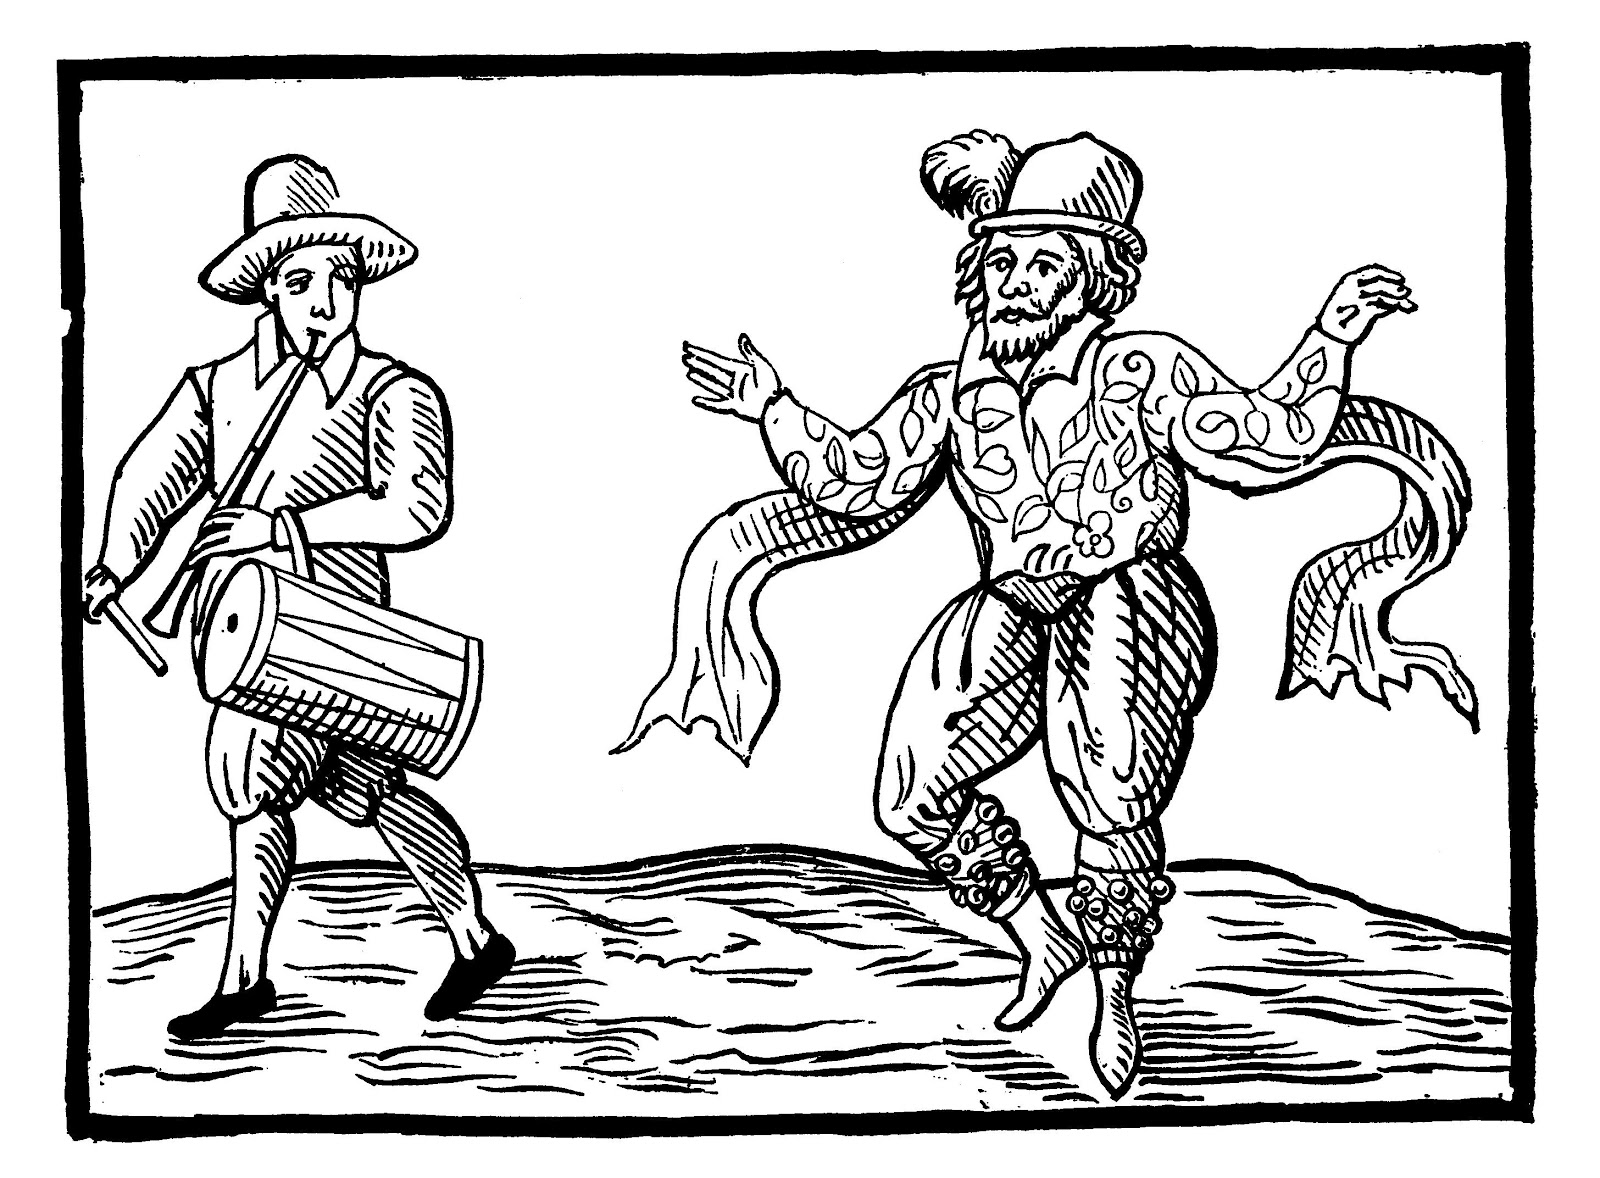
\includegraphics[width=01\textwidth]{kemp_jig.jpg}
\nbvspace[1]


\fontspec[Scale=2]{IM FELL English PRO}
HAMILTON\\

\nbvspace[0.15]

\fontspec[Scale=1.5]{IM FELL English PRO}
%Printed by Emma Badowski,\\
\nbvspace[0.1]
\fontspec[Scale=2]{IM FELL English PRO}
2 0 1 4.
\nbvspace[1]

\end{center}
\end{document}